\providecommand{\main}{../..}
\documentclass[\main/notes.tex]{subfiles}

\begin{document}
	\setcounter{chapter}{6}
	\chapter{Operational Systems}
		\section{Enterprise Resource Planning}
			\begin{definition}{Enterprise Resource Planning (ERP)}
				A system that manages an entire company's vital business information.

				Evolved from \concept{material requirements planning (MRP)}, which allowed companies to plan out how much raw material they would need at a certain time in the future, plan their production, control their inventory, and manage their purchasing process.
			\end{definition}
			\begin{sidenote}{Advantages of ERP Systems}
				\begin{description}
					\item[Improved Access to Data for Operational Decision-Making] ERP systems use an integrated database -- use one set of data to support all business functions.
					\item[Elimination of Costly, Inflexible Legacy Systems] Replace separate systems with one, single, integrated system for the entire enterprise.
					\item[Improvement of Work Processes] As ERP development is designed to support best practices, this ensures the processes are based on these.
					\item[Upgrade of Technology Infrastructure] An organisation can eliminate the multiple hardware platforms, operating systems, and databases it is currently using. This reduces ongoing maintenance.
				\end{description}
			\end{sidenote}
			\pagebreak
			\begin{sidenote}{Disadvantages of ERP Systems}
				\begin{description}
					\item[Expense and Time in Implementation] Requires time and money in order to correctly set it up, and implement it
					\item[Difficulty Implementing Change] An organisation might require radical change in the way it operates in order to use the ERP System
					\item[Difficulty Integrating With Other Systems] Hard to integrate existing systems with a new ERP system
					\item[Difficulty in Loading Data into New ERP System] Need to load data from existing systems into the new one. This is dependent on the scope of ERP implementation.
						\begin{description}
							\item[Data mapping] The examination of each data item required for the new ERP system, and determining where the data item will come from. Often requires \concept{data clean-up} afterwards.
							\item[Data loading] Performed either by using data conversion software, or by end-users entering data via input screens of the new system.
						\end{description}
					\item[Risks in Using One Vendor] After an organisation has switched to a vendor for an ERP system, the vendor has less incentive to listen and respond to customer concerns.
					\item[Risk of Implementation Failure] Implementation requires large amounts of resources, the best IS and business people, and plenty of management support.
				\end{description}
			\end{sidenote}
			\subsection{ERP for Small- and Medium-Sized Enterprises (SMEs)}
				SMEs (both for-profit and not-for-profit) can achieve benefits using ERP. Many of these elect to use \concept{open-source ERP systems}, where the source code can be seen and modified.
				\begin{center}
					\begin{tblr}{colspec={cl}, row{1}={font=\bfseries}}
						\toprule
						Vendor & ERP Solutions\\
						\midrule
						Apache & Open For Business ERP\\
						Compiere & Compiere Open Source ERP\\
						Openbravo & Openbravo Open Source ERP\\
						WebERP & WebERP\\
						\bottomrule
					\end{tblr}
				\end{center}

		\pagebreak
		\section{Transaction Processing Systems}
			Examples of transaction processing systems (TPS):
			\begin{multicols}{2}
				\begin{itemize}[nosep]
					\item Order processing
					\item Inventory Control
					\item Payroll
					\item Accounts Payable
					\item Accounts Receivable
					\item General Ledger
				\end{itemize}
			\end{multicols}
			\begin{sidenote}{Transaction Processing System}
				\begin{description}[nosep]
					\item[Input] Basic Business Transactions
					\item[Processing] Data Collection, Data Editing, Data Correction, Data Manipulation, Data Storage, Document Production
					\item[Result] Organisation's records are updated to reflect the status of the operation at the time of the last processed transaction.
				\end{description}
				Also collects data which is input to other essential information systems, where it serves as a foundation of these other systems.

				Routine operations. The support for decision-making that is directly provided is \emph{low}.
			\end{sidenote}
			\subsection{Traditional Transaction Processing Methods and Objectives}
				\begin{definition}{Batch Processing Systems}
					A form of data processing where business transactions are accumulated over a period of time and prepared for processing as a single unit or batch.

					Some delay between an event and the eventual processing of the related transaction.

					Can be more cost-effective than OLTP.
				\end{definition}
				\begin{definition}{Online Transaction Processing (OLTP)}
					A form of data processing where each transaction is processed immediately, without the delay of accumulating transactions into a batch.

					The data in an online system reflects the current status.

					Can provide faster, more efficient service.
				\end{definition}
				\begin{sidenote}{Objectives of Transaction Processing Systems}
					\begin{itemize}[nosep]
						\item Process data generated by and about transactions
						\item Maintain a high degree of accuracy and integrity
						\item Avoid processing fraudulent transactions
						\item Produce timely user responses and reports
						\item Increase labour efficiency
						\item Help improve customer service
						\item Help build and maintain customer loyalty
						\item Achieve competitive advantage
					\end{itemize}
				\end{sidenote}
			\subsection{Transaction Processing Activities}
				\begin{definition}{Transaction Processing Cycle}
					The process of data collection, data editing, data correction, data manipulation, data storage, and document production.
					\begin{center}
						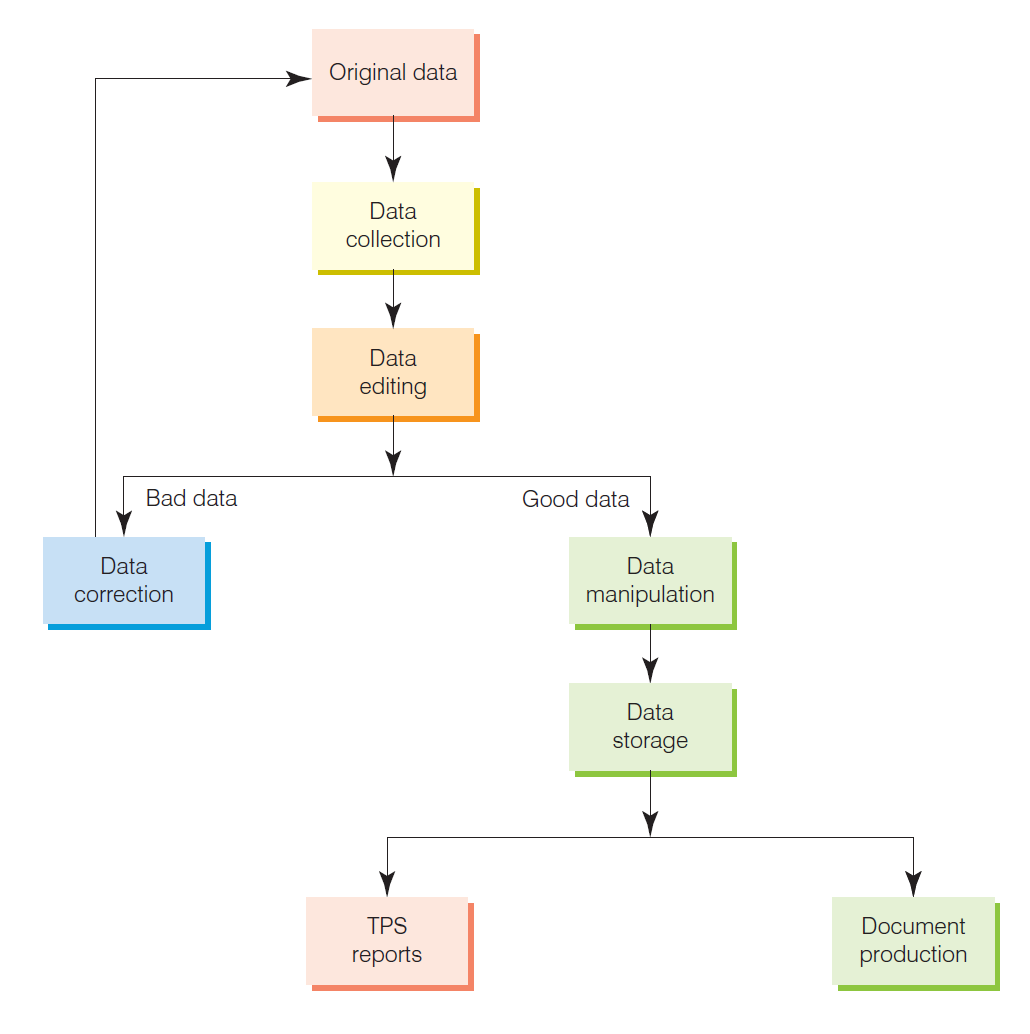
\includegraphics[width=0.75\textwidth]{chapter07/transaction_lifecycle.png}
					\end{center}
				\end{definition}
				\begin{definition}{Data Collection}
					Capturing and gathering all data necessary to complete the processing of transactions.

					Can be done manually, or automated using input devices such as barcode scanners and RFID readers. If done automatically, this is called \concept{source data automation}.

					Begins with a transaction and results in data that serves as input to the TPS.
				\end{definition}
				\begin{definition}{Data Editing}
					The process of checking data for validity and completeness.
				\end{definition}
				\begin{definition}{Data Correction}
					The process of re-entering data that was not typed or scanned properly.
				\end{definition}
				\begin{definition}{Data Manipulation}
					The process of performing calculations and other data transformations related to business transactions.
				\end{definition}
				\begin{definition}{Data Storage}
					Updating one or more databases with new transactions.
				\end{definition}
				\begin{definition}{Document Production}
					The process of generating output records and reports.
				\end{definition}
	\vbox{\rulechapterend}
\end{document}